\documentclass[sigconf,article]{acmart}

% for NTCIR proceedings
\settopmatter{printacmref=false}
\renewcommand\footnotetextcopyrightpermission[1]{}
\pagenumbering{gobble}

\usepackage{booktabs}
\usepackage{graphicx}
\usepackage{microtype}
\usepackage{xurl}
\graphicspath{{./}{paper_ntcir/}}
\setlength{\emergencystretch}{2em}

% Use one restrained booktabs style across every table.
\setlength{\heavyrulewidth}{0.55pt}
\setlength{\lightrulewidth}{0.40pt}
\setlength{\cmidrulewidth}{0.40pt}
\setlength{\aboverulesep}{0.45ex}
\setlength{\belowrulesep}{0.45ex}
\setlength{\tabcolsep}{4pt}
\renewcommand{\arraystretch}{1.08}
% Compact float and caption spacing while retaining the ACM two-column geometry.
\setlength{\textfloatsep}{8pt plus 2pt minus 2pt}
\setlength{\floatsep}{6pt plus 2pt minus 2pt}
\setlength{\intextsep}{8pt plus 2pt minus 2pt}
\setlength{\abovecaptionskip}{3pt}
\setlength{\belowcaptionskip}{0pt}

\hyphenation{RegCom-Evidence-Match Sentence-BERT MiniLM}
\newcommand{\RegComEvidenceMatch}{RegCom\-Evidence\-Match}
\newcommand{\retraug}{retrieval\allowbreak-augmented}
\newcommand{\openSource}{open\allowbreak-source}
\newcommand{\logreg}{logistic\allowbreak-regression}

\begin{document}

\title{IMNTPU at NTCIR-19 RegCom: Evidence-Aware Multilingual Retrieval and Verification for SASB-Aligned ESG Regulatory Compliance Checking}

\author{Wei Chen Huang}
\affiliation{
  \institution{National Taipei University}
  \country{Taiwan}
}
\email{wesleyseawatch@gmail.com}

\author{Hsin Ting Lu}
\affiliation{
  \institution{National Taipei University}
  \country{Taiwan}
}
\email{hsintinglubob@gmail.com}

\author{Min Yuh Day}
\authornote{Corresponding author.}
\affiliation{
  \institution{National Taipei University}
  \country{Taiwan}
}
\email{myday@gm.ntpu.edu.tw}

\begin{abstract}
Sustainability standards require evidence that is not only topically relevant but also complete, category-compatible, and expressed in the required unit. Yet multilingual ESG reports are long and semi-structured, and compliance systems must connect standard definitions with local page evidence. This study investigates retrieval-conditioned language-model verification, language- and class-specific error patterns, and the retrieval limitations that arise when extending page-level checking to full reports. We evaluate a few-shot verifier on 793 non-Chinese test rows and separately analyze a reconstructed full-report retrieval diagnostic. The best text-prompt configuration reaches Macro F1 0.6140, compared with 0.4489 for an embedding baseline; a separate low-detail page-image configuration reaches 0.5748 under a setting in which demonstrations remain text-only. In the retrieval diagnostic, a BGE-M3 multi-representation first-stage arm improves Hit@1 from 0.220 to 0.266, while a separate GPT-5.4-nano reranking run reaches 0.328; these values are not additive. Comparative and qualitative analyses identify partial disclosure and language-dependent candidate recall as persistent boundaries. The academic contribution is a reproducible evidence-matching framework and a cross-system account of accuracy--complexity trade-offs; the practical implication is a staged workflow that exposes uncertainty and routes visually complex pages to targeted review.
\end{abstract}

\keywords{ESG compliance, SASB standards, \retraug{} generation, multilingual NLP, multimodal verification}

\maketitle
\pagestyle{plain}
% Slightly compact body text to meet the nine-page submission limit.
\fontsize{8.5pt}{9.5pt}\selectfont

\section*{Team Name}
IMNTPU

\section*{Subtasks}
Subtask 1 (multilingual evidence page retrieval) and Subtask 2 (page-level three-way compliance verification), covering five official languages: English, French, Japanese, Korean, and Thai.

\section{Introduction}
\subsection{Background and Motivation}
Sustainability reporting standards require firms to disclose environmental, social, and governance (ESG) information according to specific metric definitions, disclosure categories, and units of measure. The Sustainability Accounting Standards Board (SASB) standards are representative of this metric-oriented style: a disclosure is not only about a topic, but also about whether it satisfies a precise metric, category, and unit requirement~\cite{sasb2023standards}. ESG reports are long, multilingual, and often semi-structured, so page-level compliance checking is costly for regulators, assurance providers, and analysts.

The NTCIR-19 RegCom task formulates this challenge as multinational, multilingual, and multi-industry regulatory compliance verification for ESG reports~\cite{seki2026overview,ntcir19regcom}. In Subtask 2, each instance contains a SASB metric row and a single page from an ESG report. A system must predict three fields: \texttt{pred\_label}, \texttt{category\_match}, and \texttt{unit\_match}. The main label has three values: \texttt{yes}, \texttt{yes but not complete}, and \texttt{no}. This makes the task harder than topical relevance classification. A page may discuss the same ESG topic yet fail to disclose the required quantity, omit sub-items, use a proxy, or report an incompatible unit.

Recent multilingual ESG and promise-verification studies demonstrate the value of evidence-aware analysis~\cite{seki2025mlpromise,chen2025semeval,schmoll2025automated}, while the current RegCom task emphasizes metric-level category and unit compatibility~\cite{seki2026overview}. However, most reported comparisons still leave three questions open: whether retrieval-conditioned verification is statistically better than a transparent embedding baseline, how evidence modality affects difficult partial disclosures, and how retrieval errors propagate across languages.

\subsection{Research Objective and Questions}
This study aims to develop and critically evaluate a reproducible evidence-matching workflow for multilingual SASB compliance checking. Specifically, we ask:

\begin{itemize}
\item \textbf{RQ1:} Does the complete retrieval-conditioned few-shot system improve balanced classification performance over a multilingual embedding baseline on the same page-level rows?
\item \textbf{RQ2:} How do model family, page-image evidence, disclosure class, and language change the observed performance and error patterns?
\item \textbf{RQ3:} Which lexical, dense, multi-vector, and VLM retrieval components improve full-report page localization, and where does candidate recall remain the limiting factor?
\end{itemize}

\subsection{Contributions}
We present \RegComEvidenceMatch{}, a lightweight evidence-matching verifier that uses labeled training rows as a retrieval memory and asks an LLM to make a structured page-level judgement. The design follows the intuition of few-shot prompting~\cite{brown2020language} and \retraug{} generation~\cite{lewis2020retrieval}: rather than updating model parameters, the system supplies task-relevant examples at inference time. Our contributions are fourfold. First, we provide a transparent retrieval-and-prompting design for SASB page-level verification. Second, we compare LLM and embedding-based systems under a common 793-row non-Chinese split and add paired confidence intervals and significance tests. Third, we combine quantitative ablations with language-level and case-based error analysis, including a reconstructed full-report retrieval extension. Fourth, we interpret the findings across the Cierpa and CSCU submissions and derive academic, practical, and managerial implications without treating non-aligned scores as a leaderboard. Because zero-shot and random-example controls were not run in this study, the results establish system-level performance differences rather than a causal gain attributable to retrieval alone.

We also report a cached retrieval extension toward official Subtask 1 to identify requirements for end-to-end evaluation (Section~\ref{sec:task1-diagnostic}).

\section{Related Work}
\subsection{ESG Disclosure Analysis and Multilingual Verification}
ESG analysis evaluates the completeness and reliability of sustainability disclosures~\cite{schmoll2025automated}; multilingual settings add variation in language, industry, and reporting format~\cite{li2024evaluating}. ClimateBERT and financial-report evidence extraction show the value of domain adaptation and explicit evidence~\cite{webersinke2022climatebert,kannan2023textual}. ML-Promise and SemEval-2025 Task 6 extend this perspective to multilingual promise and evidence consistency~\cite{seki2025mlpromise,chen2025semeval}. NTCIR-19 RegCom differs by requiring page-level compliance with a SASB metric, including category and unit compatibility~\cite{ntcir19regcom}; this work targets that metric-level boundary.

\subsection{Retrieval-Augmented and Embedding-Based Methods}
Our method is also related to few-shot prompting, \retraug{} generation, classical term weighting, and sentence embeddings. Large language models can perform new tasks from a small number of demonstrations~\cite{brown2020language}, and \retraug{} generation supplies task-relevant external evidence at inference time~\cite{lewis2020retrieval}. We use TF-IDF because it is a strong, transparent lexical retrieval baseline for term-weighted document matching~\cite{salton1988term}. Sentence-BERT and multilingual knowledge distillation provide efficient embedding baselines for cross-lingual semantic matching~\cite{reimers2019sentencebert,reimers2020multilingual}. \RegComEvidenceMatch{} combines these ideas by using retrieval to select few-shot cases for a structured single-page verifier.

\subsection{Comparison with Other RegCom Submissions}
Two submitted systems provide useful contrasts. Cierpa decomposes full-report checking into page retrieval and label inference, combining BM25, text and image representations, VLM descriptions, reciprocal-rank fusion, and reranking~\cite{endo2026cierpa}. Its few-shot study compares random and metric-prioritized demonstrations, but the broad pipeline requires several model calls.

CSCU emphasizes traceable evidence grounding with table-of-contents localization, fallback search, and VLM guidance~\cite{boonsuriyatham2026cscu}. It directly compares text-only, image-only, and text-plus-image evidence, whereas its strongest retrieval variant changes several stages jointly. In contrast, \RegComEvidenceMatch{} assumes the task-provided page and focuses on lightweight case retrieval and metric-level reasoning.

A terminology note is necessary: we use the official convention in which Task 1 contains Subtask 1 (full-report evidence-page retrieval) and Subtask 2 (single-page verification). Cierpa uses ``Subtask 1'' for a broader retrieval-plus-verification pipeline, so its number is not directly comparable; Section~\ref{sec:task1-diagnostic} follows the official convention.

Together these submissions suggest complementary lexical, semantic, and visual signals, but also warn that learned fusion and jointly changed VLM stages may not transfer cleanly. We use them as methodological context rather than a paired ranking; our paired tests appear in Table~\ref{tab:task2-significance} and Section~\ref{sec:task1-diagnostic}.

\begin{table*}[t]
\caption{RegCom System Design Comparison: Task Focus, Page Evidence, Full-Report Page Retrieval, Retrieved Demonstrations, and Main Trade-Offs Across Three Submissions.}
\label{tab:system-comparison}
\centering
\small
\resizebox{\textwidth}{!}{%
\begin{tabular}{llllll}
\toprule
System & Task focus & Page evidence & Page retrieval & RAG examples & Main trade-off \\
\midrule
\RegComEvidenceMatch{} & Subtasks 1--2 & Extracted text and page image & Lexical, dense, multi-vector, VLM reranking & TF-IDF, metric-first, label-balanced & Modular; end-to-end verifier coupling remains open \\
Cierpa & Subtasks 1--2 & Text and page image & Lexical, semantic, visual, VLM reranking & Random or metric-prioritized & Broad signals; higher cost \\
CSCU & Subtasks 1--2 & Text and/or page image & ToC-first, fallback, VLM guidance & Prompt-based verification & Traceable and multimodal; coupled changes \\
\bottomrule
\end{tabular}
}
\end{table*}

\section{Methods}
Subtask 2 is Single-Page Metric Verification. Given a single SASB metric and a single page from an ESG report, the objective is to determine whether that page contains relevant information and, if so, whether the information complies with the specified SASB category and unit of measure. Each instance contains structured SASB metadata, extracted page text, and three prediction targets: \texttt{pred\_label}, \texttt{category\_match}, and \texttt{unit\_match}. The main label is \texttt{yes}, \texttt{yes but not complete}, or \texttt{no}; if the prediction is \texttt{no}, the auxiliary fields are normalized to \texttt{N/A}. Because only one page is available, the task requires fine-grained local evidence matching rather than full-report compliance analysis.

The experiments use the non-Chinese subset of the task package, covering English, French, Japanese, Korean, and Thai. The retrieval and classifier training pool contains 753 labeled rows, and the evaluation set contains 793 rows. The training pool contains 295 \texttt{yes}, 127 \texttt{yes but not complete}, and 331 \texttt{no} rows, while the test set contains 315 \texttt{yes}, 138 \texttt{yes but not complete}, and 340 \texttt{no} rows.

\subsection{Proposed Research Architecture}
Figures~\ref{fig:task1-architecture} and~\ref{fig:task2-architecture} show the two task-specific research architectures. Subtask 1 starts from full ESG reports and localizes evidence pages through multi-model retrieval and VLM reranking. Subtask 2 receives one metric and one page, retrieves labeled demonstrations, and performs three-way compliance verification with text and optional page-image evidence.

\begin{figure*}[t]
\centering
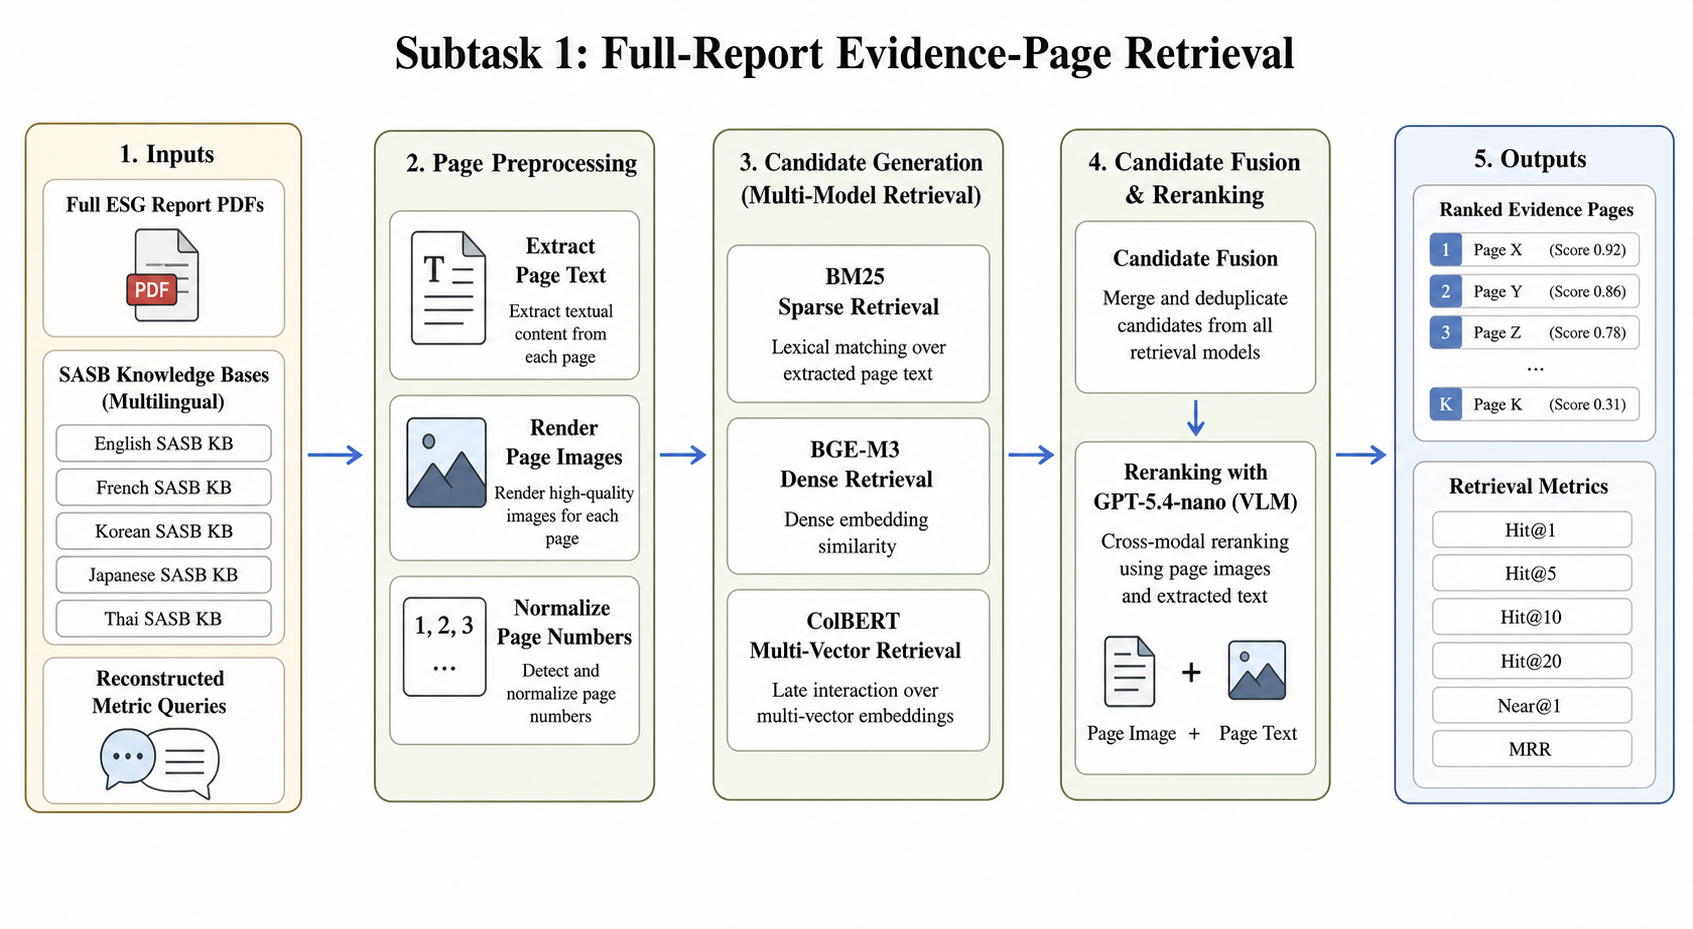
\includegraphics[width=\textwidth]{sasb_task1_architecture_generated.png}
\caption{Subtask 1 Multilingual Full-Report Evidence-Page Retrieval Architecture.}
\Description{A generated left-to-right flowchart for Subtask 1. Full ESG report PDFs, five-language SASB knowledge bases, and reconstructed metric queries are preprocessed into page text and page images. BM25, BGE-M3 dense retrieval, and ColBERT multi-vector retrieval generate candidates; candidate fusion and GPT-5.4-nano VLM reranking produce ranked evidence pages and retrieval metrics.}
\label{fig:task1-architecture}
\end{figure*}

\begin{figure*}[t]
\centering
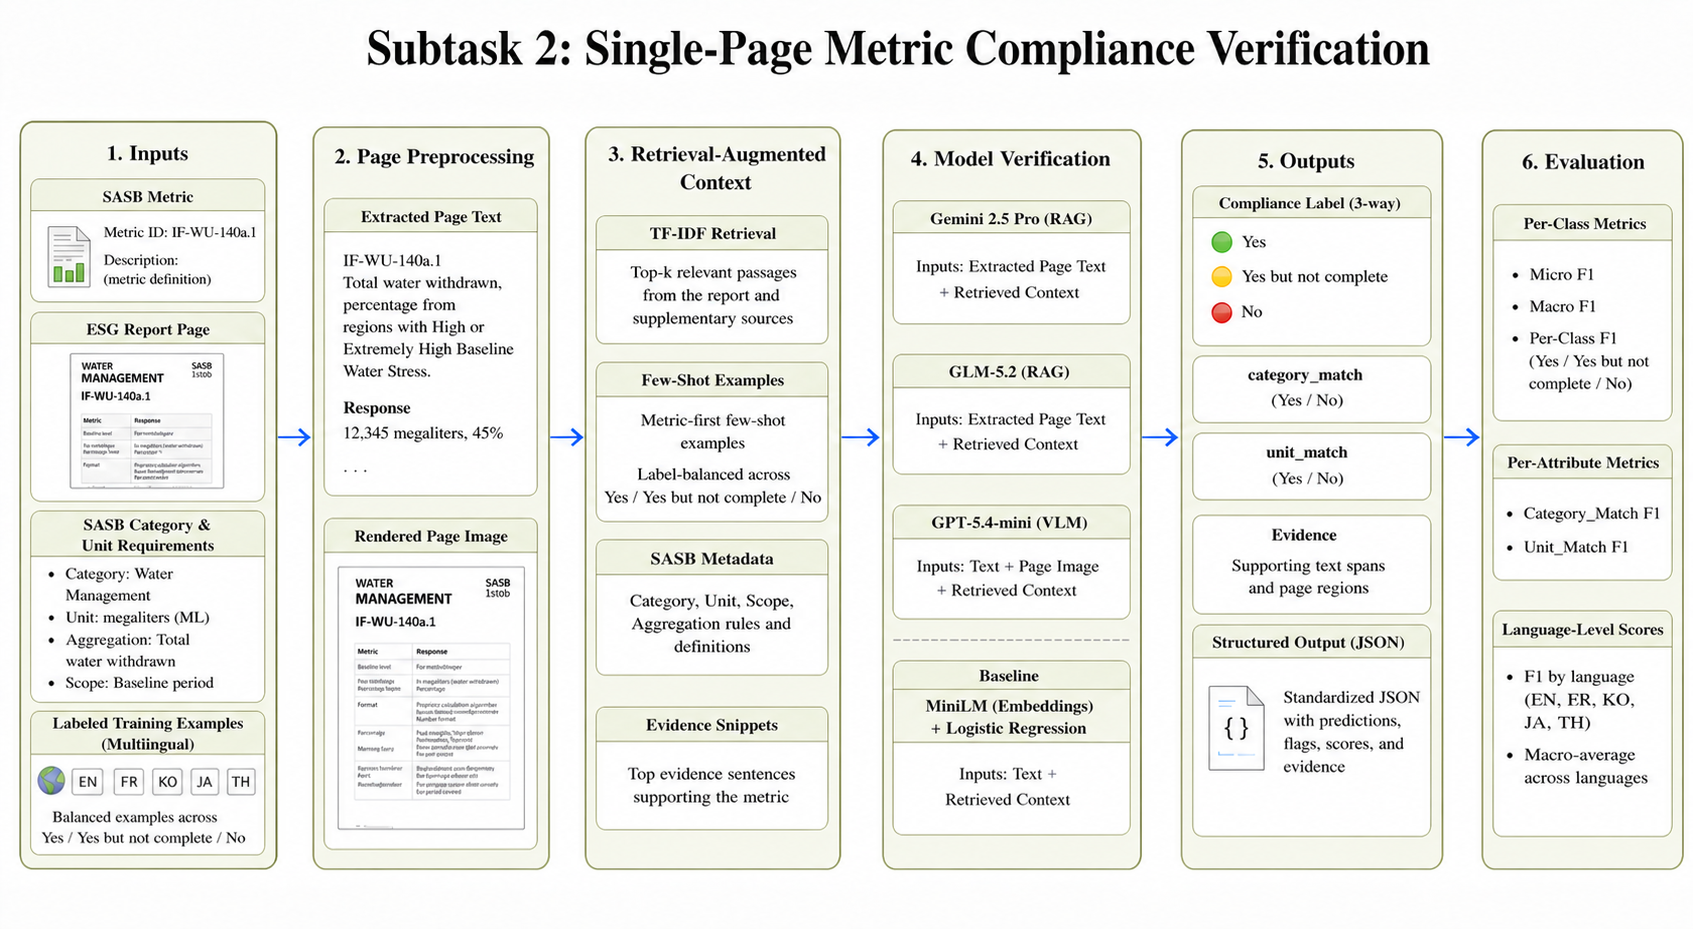
\includegraphics[width=\textwidth]{sasb_task2_architecture_generated.png}
\caption{Subtask 2 Multilingual Single-Page Metric Compliance Verification Architecture.}
\Description{A generated left-to-right flowchart for Subtask 2. One SASB metric, one ESG report page, category and unit requirements, and multilingual labeled examples are converted into extracted text and a rendered page image. TF-IDF and metric-first, label-balanced retrieval supplies context to Gemini 2.5 Pro, GLM-5.2, GPT-5.4-mini VLM, and a MiniLM logistic-regression baseline. The output is a three-way compliance label, category and unit matches, evidence, structured JSON, and class and language metrics.}
\label{fig:task2-architecture}
\end{figure*}

\subsection{Retrieval-Augmented Few-Shot Verifier}
\RegComEvidenceMatch{} does not fine-tune the LLM. Instead, it treats the training CSV as a case library. For each test row, we build a retrieval document from the SASB topic, metric description, metric code, category, unit, key terms, \texttt{sasb\_what\_counts}, and the first 1,500 characters of extracted page text. A TF-IDF vectorizer with unigram and bigram features computes cosine similarity between the test row and all training rows~\cite{salton1988term}.

The example selector retrieves three demonstrations. It first prioritizes rows with the same SASB metric code. Within that pool, it attempts to select the most similar example for each label: \texttt{yes}, \texttt{yes but not complete}, and \texttt{no}. If a label is missing for the same metric, the selector falls back to the global training pool. Remaining slots are filled by the most similar same-metric rows and then by the most similar global rows. This strategy is both similarity-based and label-balanced, reducing the chance that the prompt is dominated by the majority class.

The verifier prompt contains a compact system instruction, the retrieved demonstrations with gold outputs, the metric-specific label prior, the target SASB metadata, and the extracted PDF page text. The LLM is instructed to judge only the given page, not the full ESG report, and to return compact JSON containing \texttt{pred\_label}, \texttt{category\_match}, \texttt{unit\_match}, short evidence, and a short reason. The prompt also states the boundary rules: relevant and complete disclosure is \texttt{yes}; partial, proxy-only, incomplete, or wrong-unit disclosure is \texttt{yes but not complete}; and semantically absent metric evidence is \texttt{no}.

\subsection{Prompt Design}
The Gemini and GLM prompts share one compact schema. Each prompt tells the model to judge only the supplied page, use three retrieved demonstrations and the metric label prior for calibration, and return JSON containing \texttt{pred\_label}, \texttt{category\_match}, \texttt{unit\_match}, evidence, and reason. The rules distinguish complete, partial/proxy or wrong-unit, and absent disclosures; an absent prediction sets the auxiliary fields to \texttt{N/A}. The target row includes language, report and page identifiers, metric metadata, SASB category and unit, key terms, ``what counts'' guidance, and extracted page text.

\begin{quote}\small\itshape
Judge only the supplied PDF page. Given the SASB metric, category/unit requirements, page text, and three retrieved labeled examples, return compact JSON with \texttt{pred\_label}, \texttt{category\_match}, \texttt{unit\_match}, evidence, and reason. Use \texttt{yes} for complete evidence, \texttt{yes but not complete} for partial/proxy/wrong-unit evidence, and \texttt{no} when the metric is absent; set auxiliary fields to \texttt{N/A} for \texttt{no}.
\end{quote}

\iffalse
\begin{quote}\small\itshape
You are a SASB page-level verification assistant. Judge only the single PDF page provided. Return compact JSON only with the following fields:

\texttt{\{"pred\_label": "yes|yes but not complete|no",}\\
\texttt{"category\_match": "yes|no|N/A",}\\
\texttt{"unit\_match": "yes|no|N/A",}\\
\texttt{"evidence": "short page evidence",}\\
\texttt{"reason": "short reason"\}}

Rules:\\
1. Predict \texttt{yes} if the page contains relevant disclosure for the requested SASB metric.\\
2. Predict \texttt{yes but not complete} if the page is relevant but partial, proxy-only,\\
   incomplete, or wrong-unit.\\
3. Predict \texttt{no} if the exact metric is not semantically disclosed.\\
4. If \texttt{pred\_label} is \texttt{no}, set \texttt{category\_match} and\\
   \texttt{unit\_match} to \texttt{N/A}.\\
5. Use the retrieved few-shot examples and metric label distribution only as calibration. The target page evidence decides.

Retrieved few-shot examples:\\
Example 1--3: task metadata, evidence snippet, similarity score, same-metric flag, and gold output.

Now predict this test row:\\
Task: language, company/report id, file stem, page, metric code, topic, metric description, SASB category, unit, key terms, and what-counts guidance.\\
PDF page text: [extracted page text, truncated to 5,000 characters]\\
Return JSON only.
\end{quote}
\fi

Each retrieved example contains an evidence snippet (up to 1,200 characters), similarity score, same-metric flag, and gold output; the prompt also supplies a same-metric label prior. Invalid auxiliary labels are normalized deterministically. Narrative evidence is treated as category- and unit-compatible for discussion-and-analysis metrics, and zero-event statements can satisfy event-count metrics.

\subsection{Compared Systems}
We evaluate Gemini 2.5 Pro and GLM-5.2 with the same retrieval, prompt, structured task fields, page text, and three demonstrations. Gemini provides advanced reasoning, multimodality, and long-context processing~\cite{gemini2025gemini25}; GLM-5.2 provides an alternative multilingual instruction-following model~\cite{zeng2024chatglm}.

As a multimodal follow-up, GPT-5.4-mini receives the target page at 96 DPI as a low-detail image plus extracted text; demonstrations remain text-only. It is evaluated on the same 793 rows as a configuration comparison, not a replacement for Gemini/GLM.

As a lightweight \openSource{} baseline, we encode the same page representation with multilingual MiniLM~\cite{wang2020minilm,reimers2019sentencebert,reimers2020multilingual} and train balanced logistic regression~\cite{pedregosa2011scikit} for the three labels. Auxiliary fields are derived deterministically; this fast baseline does not explicitly reason about completeness, units, or page boundaries.

\subsection{Evaluation Metrics}
Micro F1 and Macro F1 are the primary metrics. Macro F1 averages class-wise F1 and is important because \texttt{yes but not complete} is less frequent but central to compliance. The retrieval extension additionally reports exact hits, Near@1, candidate recall, and MRR. Because no independently validated categorical gold is available for \texttt{category\_match} and \texttt{unit\_match}, we score \texttt{pred\_label} and treat these fields as format-normalized outputs.

\subsection{Statistical Validation}
We align Task 2 predictions by language, report, metric, page, and file stem (with an occurrence index for duplicates). Pairwise comparisons on the same 793 rows use exact McNemar tests and 10,000 paired bootstrap resamples for accuracy and Macro F1; six $p$-values receive Holm correction at $\alpha=0.05$. The reconstructed Task 1 comparisons use the same paired procedures on 369 non-empty-gold groups.

\subsection{Qualitative and User-Oriented Evaluation}
We analyze cached traces for improvements, regressions, candidate-recall misses, index-page confusions, and language-specific failures. The 65-row stratified sample is reserved for future double annotation; no human user study is claimed here. A planned user evaluation would compare text-only and multimodal evidence on identical cases using accuracy, review time, calibration, and trust.

\section{Experiments}
\subsection{Overall Results}
Table~\ref{tab:overall} reports the overall results. Gemini 2.5 Pro achieves the best score, with 0.6507 Micro F1 and 0.6140 Macro F1. GLM-5.2 is close, with 0.6280 Micro F1 and 0.5963 Macro F1. GPT-5.4-mini with a low-detail page image obtains 0.6217 Micro F1 and 0.5748 Macro F1, below the two text-prompt LLM configurations in this run but well above MiniLM. MiniLM with logistic regression is much faster but substantially weaker, with 0.4603 Micro F1 and 0.4489 Macro F1. These results indicate that retrieval-conditioned LLM verification adds meaningful value beyond multilingual semantic embeddings, while a single low-detail image does not automatically improve the decision boundary for partial disclosures.

\begin{table}[t]
\caption{Task 2 Single-Page Metric Verification: Overall Micro F1 and Macro F1 for Four Models on 793 Non-Chinese Test Rows.}
\label{tab:overall}
\centering
\begin{tabular}{lrr}
\toprule
System & Micro F1 & Macro F1 \\
\midrule
Gemini 2.5 Pro RAG & \textbf{0.6507} & \textbf{0.6140} \\
GLM-5.2 RAG & 0.6280 & 0.5963 \\
GPT-5.4-mini VLM & 0.6217 & 0.5748 \\
MiniLM + LR & 0.4603 & 0.4489 \\
\bottomrule
\end{tabular}
\end{table}

\begin{figure*}[t]
\centering
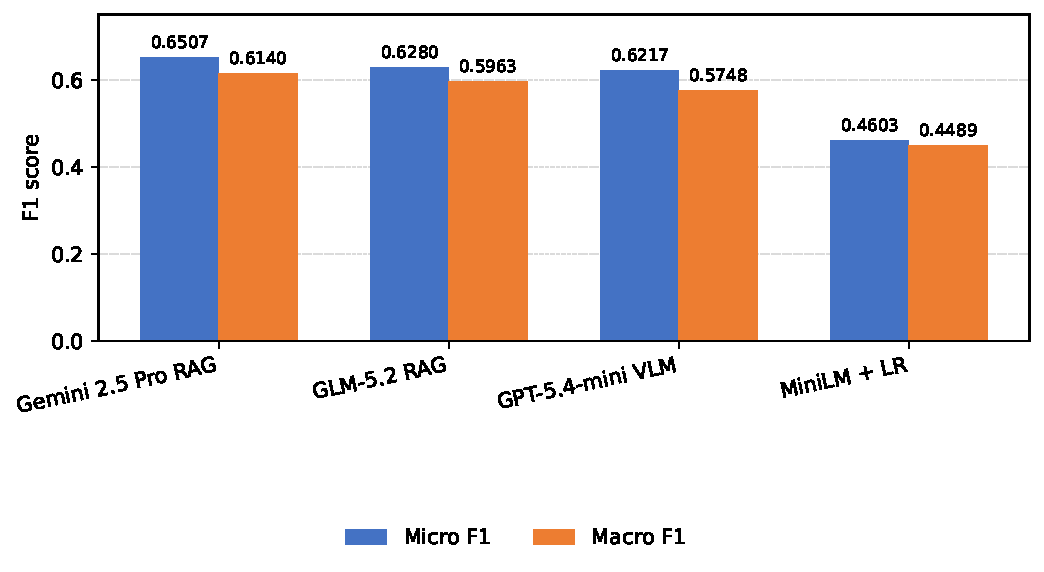
\includegraphics[width=0.94\textwidth]{task2_model_score_comparison.pdf}
\caption{Task 2 Single-Page Metric Verification: Micro F1 and Macro F1 by Model on the 793 Non-Chinese Test Rows.}
\Description{A grouped vertical bar chart comparing Gemini 2.5 Pro RAG, GLM-5.2 RAG, GPT-5.4-mini VLM, and MiniLM plus logistic regression on Task 2. Gemini has the highest Micro F1 and Macro F1, followed by GLM-5.2, GPT-5.4-mini, and MiniLM.}
\label{fig:task2-model-bars}
\end{figure*}

\begin{table*}[t]
\caption{Paired Task 2 Model Comparisons on Identical Non-Chinese Rows: Accuracy and Macro F1 Differences with 95\% Paired Bootstrap Confidence Intervals and Holm-Adjusted Exact McNemar $p$-Values for Accuracy.}
\label{tab:task2-significance}
\centering
\scriptsize
\resizebox{\textwidth}{!}{%
\begin{tabular}{lrrrrr}
\toprule
Comparison & $\Delta$ Accuracy & 95\% CI & $\Delta$ Macro F1 & 95\% CI & Holm $p$ (accuracy) \\
\midrule
Gemini--GLM & +0.0227 & [-0.0025, 0.0492] & +0.0177 & [-0.0137, 0.0502] & 0.209 \\
Gemini--GPT-5.4-mini & +0.0293 & [-0.0025, 0.0618] & +0.0395 & [-0.0000, 0.0795] & 0.294 \\
Gemini--MiniLM & +0.1907 & [0.1488, 0.2358] & +0.1653 & [0.1204, 0.2111] & $<0.001^{***}$ \\
GLM--GPT-5.4-mini & +0.0066 & [-0.0240, 0.0366] & +0.0218 & [-0.0119, 0.0553] & 0.748 \\
GLM--MiniLM & +0.1680 & [0.1261, 0.2119] & +0.1476 & [0.1058, 0.1916] & $<0.001^{***}$ \\
GPT-5.4-mini--MiniLM & +0.1614 & [0.1185, 0.2055] & +0.1259 & [0.0814, 0.1702] & $<0.001^{***}$ \\
\bottomrule
\end{tabular}
}
\par\smallskip\noindent\footnotesize\emph{Note:} $^{*}p<0.05$, $^{**}p<0.01$, and $^{***}p<0.001$; stars mark two-sided exact McNemar tests after Holm correction across the six pairwise comparisons.
\end{table*}

The paired tests qualify the apparent ranking in Table~\ref{tab:overall}. After Holm correction across the six comparisons, each LLM configuration is significantly better than MiniLM on correctness, whereas the Gemini--GLM and Gemini--GPT-5.4-mini differences are not statistically significant at $\alpha=0.05$. Thus, the point estimate favors Gemini, but the available paired evidence supports a robust LLM-versus-embedding contrast rather than a conclusive winner among the LLMs. The full row-alignment and resampling record is provided in \texttt{artifacts/metrics/task2\_paired\_significance.json}.

\subsection{Class-Level Results}
Table~\ref{tab:class} shows class-level F1. The \texttt{no} class is strongest for both LLM systems, while \texttt{yes but not complete} remains the weakest class. Gemini reaches 0.4835 F1 on \texttt{yes but not complete}; GLM-5.2 reaches 0.4717; MiniLM reaches 0.3931. GLM-5.2 has higher recall on the partial class, but lower precision, suggesting that it more often uses the partial label as a cautious middle state. Gemini is more conservative on partial predictions and obtains better overall balance.

\begin{table}[t]
\caption{Task 2 Single-Page Metric Verification: F1 Scores for the \texttt{yes}, \texttt{yes but not complete}, and \texttt{no} Prediction Classes on the Non-Chinese Test Set.}
\label{tab:class}
\centering
\begin{tabular}{lrrr}
\toprule
System & yes & ybnc & no \\
\midrule
Gemini 2.5 Pro RAG & \textbf{0.6327} & \textbf{0.4835} & \textbf{0.7258} \\
GLM-5.2 RAG & 0.5919 & 0.4717 & 0.7250 \\
GPT-5.4-mini VLM & 0.6266 & 0.3686 & 0.7292 \\
MiniLM + LR & 0.5133 & 0.3925 & 0.4411 \\
\bottomrule
\end{tabular}
\begin{flushleft}
\small Note: ybnc = \texttt{yes but not complete}.
\end{flushleft}
\end{table}

\subsection{Language-Level Results}
Language-level results are shown in Table~\ref{tab:lang}. Gemini is strongest on French, Japanese, and Korean. Gemini and GLM-5.2 tie on Thai Micro F1, while GLM-5.2 has the highest Thai Macro F1. GPT-5.4-mini is strongest on English (Micro F1 0.6269 and Macro F1 0.5802), where Gemini is comparatively weakest; GPT-5.4-mini remains below Gemini on the other four languages. MiniLM is consistently below the LLM systems, with the largest gap on Thai.

\begin{table}[!t]
\caption{Task 2 Single-Page Metric Verification: Language-Level Micro F1 and Macro F1 for English, French, Japanese, Korean, and Thai.}
\label{tab:lang}
\centering
\scriptsize
\resizebox{\columnwidth}{!}{%
\begin{tabular}{llrrrrr}
\toprule
System & Metric & English & French & Japanese & Korean & Thai \\
\midrule
Gemini 2.5 Pro RAG & Micro F1 & 0.5473 & \textbf{0.6771} & \textbf{0.7231} & \textbf{0.7718} & \textbf{0.5537} \\
 & Macro F1 & 0.4833 & \textbf{0.6382} & \textbf{0.6801} & \textbf{0.7467} & 0.5129 \\
GLM-5.2 RAG & Micro F1 & \textbf{0.5473} & 0.6406 & 0.6538 & 0.7584 & \textbf{0.5537} \\
 & Macro F1 & \textbf{0.5090} & 0.5971 & 0.5996 & 0.7337 & \textbf{0.5180} \\
GPT-5.4-mini VLM & Micro F1 & 0.6269 & 0.6354 & 0.6077 & 0.6711 & 0.5455 \\
 & Macro F1 & 0.5802 & 0.5825 & 0.5555 & 0.6321 & 0.4864 \\
MiniLM + LR & Micro F1 & 0.4726 & 0.5104 & 0.4846 & 0.4430 & 0.3554 \\
 & Macro F1 & 0.4550 & 0.4548 & 0.4767 & 0.4388 & 0.3100 \\
\bottomrule
\end{tabular}
}
\end{table}

\subsection{Cross-Submission Comparison}
Table~\ref{tab:reported-comparison} contextualizes our strongest result with the independently reported Subtask 2 results from Cierpa and CSCU. Cierpa reports an overall Macro F1 of 0.637 for its best metric-aware few-shot configuration across six languages~\cite{endo2026cierpa}. CSCU reports 0.624 Macro F1 and 67.9\% accuracy for text-plus-image verification over 967 retained page records~\cite{boonsuriyatham2026cscu}. Our Gemini configuration reports 0.614 Macro F1 and 65.07\% Micro F1 over 793 non-Chinese rows; the additional GPT-5.4-mini VLM run reports 0.5748 Macro F1 and 62.17\% accuracy on the same rows.

These values are close in magnitude but are not directly comparable. Our evaluation excludes Chinese, Cierpa applies a conflict-oriented cleaning procedure, and CSCU reports a retained 967-record set and excludes a documented source-alignment anomaly. The systems also differ in model, prompt, page modality, and example selection. Consequently, Table~\ref{tab:reported-comparison} is a comparison of reported experimental contexts rather than an official ranking or a paired significance test.

\begin{table}[t]
\caption{Cross-Submission Context: Independently Reported Best Subtask 2 Results with Evaluation Scope and Retained-Row Differences.}
\label{tab:reported-comparison}
\centering
\small
\resizebox{\columnwidth}{!}{%
\begin{tabular}{lrrl}
\toprule
System & Macro F1 & Acc./Micro F1 & Scope \\
\midrule
Cierpa Best F1 & 0.637 & -- & Six languages, cleaned \\
CSCU text+image & 0.624 & 0.679 & 967 retained rows \\
\RegComEvidenceMatch{} Gemini & 0.614 & 0.6507 & 793, no Chinese \\
\RegComEvidenceMatch{} GPT-5.4-mini VLM & 0.5748 & 0.6217 & 793, no Chinese \\
\bottomrule
\end{tabular}
}
\end{table}

\subsection{Result Analysis}
The main finding is that the task benefits from explicit LLM-based verification. MiniLM embeddings capture broad multilingual similarity, but the task requires more than semantic closeness. The model must decide whether a page satisfies a specific SASB metric, whether the disclosure is complete, and whether the unit is compatible. This explains why the embedding classifier often fails despite using the same training rows and PDF text.

The comparison between Gemini 2.5 Pro and GLM-5.2 also illustrates that prompt-calibrated retrieval does not remove model-specific decision tendencies. GLM-5.2 predicts \texttt{yes but not complete} more frequently, which improves recall for partial disclosures but reduces precision. Gemini 2.5 Pro predicts \texttt{no} more often and obtains stronger overall F1 balance. GPT-5.4-mini with a low-detail page image is substantially stronger than MiniLM overall, but its partial-disclosure F1 (0.3686) remains below both text-prompt LLMs. This comparison is confounded: only the target page image was added, the demonstrations remained text-only, and image resolution/detail were fixed at 96 DPI/low detail. It therefore measures one multimodal configuration rather than the isolated causal contribution of page images. In practical compliance screening, the preferred model may depend on whether the user values recall for partial disclosures or conservative final acceptance.

The other submissions refine this interpretation. Cierpa reports that metric-prioritized few-shot examples improve its aggregate score over zero-shot inference, but the effect varies by language, with gains in some slices and reversals in others. Thus, examples can calibrate a difficult boundary but can also anchor the verifier to inappropriate edge cases. This observation supports our use of same-metric examples while motivating the missing zero-shot and random-example controls.

CSCU provides complementary evidence about input modality: its text-plus-image setting outperforms text-only, although image-only and text-plus-image intervals overlap. This suggests that visual evidence can recover structure lost during extraction, but it does not identify the isolated contribution of an image under our different prompt, resolution, and model settings. Demonstration relevance and evidence fidelity therefore address different failure sources: the former calibrates the decision boundary, whereas the latter determines whether the required value, unit, and scope are visible.

Cierpa's end-to-end analysis further shows that retrieval and label inference can compound errors when page--metric labels are non-unique. A correctly retrieved page may still be scored against a mismatched page label when the same report contains both positive and negative instances for one metric. Any future end-to-end version of \RegComEvidenceMatch{} should therefore preserve row-level identity and avoid attributing every chained error to retrieval alone.

\subsection{Error Analysis}
Errors remain concentrated around partial disclosure. A page may contain relevant ESG language but omit a required denominator, scope, disaggregation, event count, or unit. Conversely, a page may present a SASB index that names a metric but does not contain the underlying disclosure. Single-page evaluation makes these cases difficult because evidence may appear on neighboring pages. The current system also relies on extracted PDF text; tables or figures that are poorly extracted may be underused.

The observed errors can be summarized into three common patterns. First, topical matches are sometimes confused with compliant disclosures: the page discusses the correct ESG issue but does not provide the metric-specific quantity, category, or unit. Second, partial disclosures are hard to separate from complete disclosures when the page provides proxy evidence, percentages without denominators, or qualitative descriptions without the required numerical detail. Third, extracted text from PDF tables may lose row or column structure, making it difficult for the verifier to connect a number with the correct SASB metric.

These patterns recur across submissions. Cierpa reports that few-shot examples improve some language-level partial-disclosure results but reverse in others, indicating that the \texttt{yes but not complete} boundary is sensitive to demonstration choice. CSCU likewise identifies this label as the hardest class and attributes remaining errors to incomplete page evidence and confusion between full and partial disclosure. Its Subtask 1 analysis additionally shows that many retrieval errors fall on a page adjacent to the annotated page. Although our system receives the official target page and does not evaluate retrieval, this finding exposes a limitation of strict single-page verification: the verifier can be penalized for missing evidence that is structurally associated with the target disclosure but printed on a neighboring page. A consolidated, cross-method error taxonomy and worked examples are provided as supplementary error-analysis material.

\subsection{Task 1 Retrieval Extension}
\label{sec:task1-diagnostic}
The RegCom shared task also defines Subtask 1 as full-report compliance matching: a system must localize relevant pages and then verify the disclosure category and unit. The experiments above do not evaluate that setting because Subtask 2 supplies the task-provided page directly. We therefore reconstruct report--metric query groups from the available page-level files and evaluate the page-localization stage separately.\footnote{Full run configurations, dates, and the claim-boundary policy are maintained in \texttt{docs/EXPERIMENT\_LOG.md} and \texttt{docs/TASK1\_VLM\_PLAN.md} in the project repository.} Since the official Subtask 1 input records, gold page sets, empty/no-disclosure rules, and evaluator are not included in this checkout, the scores below should be interpreted as reconstructed retrieval measurements rather than official leaderboard values.

The retrieval pipeline follows the general shape of Cierpa's retrieval design (Section~2.5): independent lexical and dense candidate generators, weighted reciprocal-rank fusion, a lane-union candidate pool, and Top-10 vision-language-model (VLM) reranking, evaluated against the reconstructed query groups. On 490 report--metric groups (369 with at least one non-empty gold page, 121 without), the frozen 10-candidate dense-fused configuration reaches Hit@1 0.220, Hit@5 0.493, Hit@10/candidate recall 0.631, and MRR 0.350 on the non-empty groups. A separate \texttt{gpt-5.4-nano} reranking run over those same 10 candidates reaches Hit@1 0.328, Hit@5 0.583, and MRR 0.431; these are not additive with the local BGE-M3 ablation reported below, and Hit@10 remains 0.631 because reranking cannot recover a page absent from the candidate pool. The dense-fused 10-candidate candidate recall@10 varies sharply by language (English 0.891, French 0.840, Korean 0.686, Chinese 0.576, Japanese 0.545, Thai 0.313), which identifies Thai, Chinese, and Japanese candidate generation, rather than reranking quality, as the current bottleneck. The 490 VLM traces completed successfully after rate-limit retries, using 6,758,052 input and 143,304 output tokens at an estimated cost of US\$1.531. A separate cached verifier trace produced a predicted-label distribution of 301 \texttt{no}, 143 \texttt{yes but not complete}, and 46 \texttt{yes}; only a small 74-row subset joined unambiguously to available truth after accounting for label non-uniqueness, so we do not treat that exploratory accuracy as a general Task 1 estimate.

A deeper-candidate follow-up configuration (\texttt{task1-neighbor2}: the same dense-enabled fusion, plus a two-page neighbor expansion around the Top-10 anchors, doubling the VLM candidate pool to Top-20) was completed on all 490 groups. The neighbor2 candidate-pool recall reaches 0.710 at Top-20 (0.789 at Top-30), while its 20-image nano reranker reaches Hit@1 0.314, Hit@5 0.561, Hit@10 0.648, Near@1 0.398, and MRR 0.423, compared with Hit@1/5/10 0.328/0.583/0.631 and MRR 0.431 for the 10-image primary configuration. The larger pool therefore improves coverage at Hit@10 but slightly reduces Top-1 and MRR. The effect is language-dependent: Chinese, Japanese, Korean, and Thai Top-1 improve in the 20-image neighbor2 run (e.g.\ Japanese 0.182 to 0.309), but French Top-1 regresses from 0.320 to 0.300 (MRR 0.484 to 0.467) even though French candidate recall rises from 0.840 in the 10-image primary run to 0.900 in neighbor2. Consequently neither configuration strictly dominates the other. The complete neighbor2 run used 13,178,046 input and 275,396 output tokens at an estimated cost of US\$2.980.

The completed local BGE-M3 ablation uses the same reconstructed query groups and page mapping and runs without API calls. It compares dense retrieval, dense+sparse fusion, dense+sparse+ColBERT multi-vector fusion, and BGE-Reranker-v2-M3 reranking. Table~\ref{tab:task1-bge} reports the unified scores on the 369 query groups with non-empty gold pages; the full reconstructed input contains 490 groups, including 121 empty-gold groups.

\begin{table*}[t]
\caption{Task 1 Reconstructed Full-Report Page Retrieval: Ablation Results for Five Retrieval Configurations on 369 Non-Empty-Gold Query Groups.}
\label{tab:task1-bge}
\centering
\small
\setlength{\tabcolsep}{9pt}
\renewcommand{\arraystretch}{1.15}
\begin{tabular}{lrrrrrr}
\toprule
Configuration & Hit@1 & Hit@5 & Hit@10 & Hit@20 & Near@1 & MRR \\
\midrule
MiniLM fused baseline & 0.220 & 0.493 & 0.631 & 0.751 & 0.293 & 0.350 \\
BGE-M3 dense & 0.238 & 0.504 & 0.631 & 0.748 & 0.290 & 0.369 \\
BGE-M3 dense+sparse & 0.249 & 0.523 & 0.648 & 0.772 & 0.312 & 0.381 \\
BGE-M3 dense+sparse+ColBERT & \textbf{0.266} & \textbf{0.545} & \textbf{0.675} & \textbf{0.818} & \textbf{0.325} & \textbf{0.398} \\
BGE-Reranker-v2-M3 (raw, all languages) & 0.160 & 0.504 & 0.672 & -- & -- & 0.313 \\
\bottomrule
\end{tabular}
\end{table*}

\begin{figure*}[t]
\centering
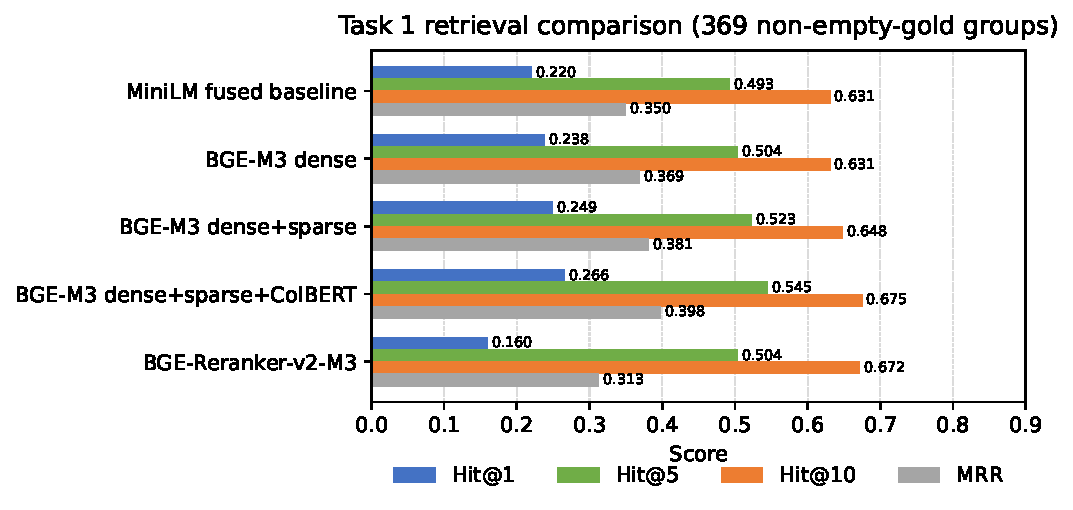
\includegraphics[width=0.94\textwidth]{task1_retrieval_score_comparison.pdf}
\caption{Task 1 Reconstructed Full-Report Page Retrieval: Hit@1, Hit@5, Hit@10, and MRR by Retrieval Configuration on 369 Non-Empty-Gold Query Groups.}
\Description{A grouped vertical bar chart comparing five Task 1 retrieval configurations: a MiniLM fused baseline, BGE-M3 dense, BGE-M3 dense plus sparse, BGE-M3 dense plus sparse plus ColBERT, and BGE-Reranker-v2-M3. The three-representation BGE-M3 configuration has the highest Hit at 1, Hit at 5, Hit at 10, and MRR, while the generic BGE reranker has the lowest Hit at 1 and MRR.}
\label{fig:task1-retrieval-bars}
\end{figure*}

The best first-stage configuration is the three-representation BGE-M3 fusion, improving over the MiniLM baseline by 4.6, 5.2, and 4.4 percentage points on Hit@1, Hit@5, and Hit@10, respectively, and by 0.048 MRR. The gains are consistent with the component ablation: sparse features add about one point over dense-only retrieval, and the ColBERT-style multi-vector lane adds a further 1.5--2 points. Natural-language query rewrites underperform the original metric-keyword queries (0.209--0.228 Hit@1 across the tested variants), suggesting that the added English ``what counts'' wording introduces noise for non-English reports. Increasing the BGE maximum length from 2,048 to 8,192 tokens has almost no effect because most page texts are shorter than the limit. In contrast, the BGE-Reranker-v2-M3 arm lowers pooled Top-1 and MRR to 0.160 and 0.313: it often promotes SASB/GRI index pages that mention a metric code over the page containing the actual disclosure. Language-specific results show the largest Top-1 gains for Korean (0.216 to 0.373) and Japanese (0.182 to 0.236); in the BGE-M3 three-representation/raw arm, Thai Hit@10 is 0.281 and remains the principal candidate-generation bottleneck. These findings support stronger multilingual candidate generation, but also show that reranking quality and disclosure-page relevance must be analyzed separately. A 65-row stratified, human-review-only error sample is provided as supplementary material; its qualitative judgment columns intentionally remain blank for manual annotation.

To quantify uncertainty, we used 10,000 paired bootstrap resamples over the same 369 non-empty groups. The best BGE fusion improves Hit@1, Hit@5, Hit@20, and MRR significantly relative to the baseline, while the positive Hit@10 and Near@1 differences include zero in their 95\% intervals. A paired McNemar test on Hit@1 gives 22 baseline-only versus 39 BGE-only successes ($p=0.040$). The raw-versus-natural query comparison is significant for the multi-vector system (22 versus 8, $p=0.016$), and the all-language reranker significantly degrades Top-1 (58 versus 25, $p=0.0004$); language gating recovers a significant portion of those errors (14 versus 48, $p<0.001$).

The error analysis separates candidate recall from ranking. The reranker selects a SASB/GRI index page as Top-1 for 91/369 raw queries (66 are incorrect) and 142/369 natural queries (111 incorrect). Representative failures include an esun query whose gold page 14 is replaced by a GRI index at page 195, and two hyundai metrics whose gold pages 72--73 are both replaced by the same SASB index at page 114. Thai and French fail for different reasons: the BGE-M3 three-representation/raw arm has Thai Hit@10 of 0.281, and the 20-image neighbor2 VLM pool misses the Thai gold page from Top-20 for 32/64 groups; by contrast, the 10-image primary VLM run has French candidate recall@10 of 0.840, neighbor2 raises it to 0.900, and the primary run's French Hit@10 is 0.860, so the dominant French issue is ordering rather than recall (29/50 gold pages are in Top-20 but not Top-1). The 121 empty-gold groups also expose a limitation of the current interface: the retriever always returns candidates, so abstention detects 0/121 cases, and the fused Top-1 score has AUC 0.48 for distinguishing empty from non-empty groups. Finally, three out-of-range gold pages in the SPT report are caused by a one-page extraction failure; because every arm uses the same page map, they affect comparisons equally.

\section{Discussion}
\subsection{Strengths and Weaknesses across Approaches}
The cross-system comparison is summarized by three complementary strengths: our method is lightweight and reproducible, Cierpa combines broad lexical, semantic, and visual retrieval, and CSCU emphasizes traceable evidence and modality analysis. Their corresponding limitations are scope and missing retrieval controls in our study, higher pipeline cost and language-dependent gains for Cierpa, and jointly changed stages and adjacent-page sensitivity for CSCU.

Cierpa offers broad complementary lexical, semantic, and visual signals but requires multiple model calls; CSCU emphasizes traceable evidence and modality analysis, although its strongest VLM variant changes several stages jointly. These observations motivate our staged, explicitly confounded multimodal comparison.

\subsection{Evaluation Scope and Validity}
Macro F1 is more informative than accuracy alone because the partial class is less frequent and consistently difficult. Nevertheless, a single aggregate score hides material differences in language coverage, class distribution, evidence quality, and retained records. Cross-submission scores should therefore be accompanied by their evaluation scope, as in Table~\ref{tab:reported-comparison}, and should not be compared as if generated on an identical paired sample.

The released reference data also complicate evaluation. Cierpa's own audit of the official release quantifies this: across all six languages, 21.1\% of training and 16.5\% of test relevant-page targets are non-unique for the same metric tuple, and 55.6\% of training and 57.2\% of test instances share a non-unique gold label at the PDF level, because a \texttt{no} label marks absence from one page rather than from the whole report. An evaluator that joins rows only by a non-unique tuple can collapse instances and change the reported result. Reviewer-facing analysis should preserve row-level identity or introduce a unique sample identifier. Separately, CSCU's audit of the official Subtask 1 split found that all official test documents also appear in the training split, which it reports as seen-document, unseen-query evaluation rather than unseen-document generalization; because Cierpa, CSCU, and \RegComEvidenceMatch{} all draw on the same official RegCom release, this framing plausibly applies to the other submissions' splits as well, though we have not independently confirmed it for the non-Chinese CSV split used here. Moreover, the available reference files do not provide independently validated gold labels for the predicted \texttt{category\_match} and \texttt{unit\_match} fields; these auxiliary outputs should not be scored by treating an answer-unit string as an equivalent categorical gold label.

Finally, exact single-page evaluation is intentionally controlled but does not represent every real report. Tables may continue across pages, narrative definitions may precede a numerical table, and SASB index pages may point to rather than contain evidence. Future evaluation could complement exact-page labels with acceptable page sets, neighboring-page sensitivity, or short evidence-span annotations. These alternatives should supplement rather than silently replace the official protocol.

\subsection{Implications for System Design}
The comparison suggests a modular research direction. Metric-prioritized examples can improve decision calibration, while page images can improve evidence fidelity; neither substitutes for the other. A practical extension of \RegComEvidenceMatch{} would preserve its lightweight text path for narrative pages and route table-heavy, scanned, or low-text pages to a multimodal verifier. A controlled ablation among zero-shot, random few-shot, TF-IDF few-shot, and metric-prioritized few-shot settings would then isolate the contribution of retrieval separately from the underlying LLM. Such experiments are preferable to attributing all gains to ``RAG'' when the model, prompt, sample scope, and evidence modality also differ.

\subsection{Limitations}
\label{sec:limitations}
Our conclusions are subject to several limitations. First, our primary results cover 793 non-Chinese rows and therefore do not constitute a complete six-language evaluation. Second, Gemini 2.5 Pro and GLM-5.2 are remote models whose behavior and availability may change, while exact generation-level seeds and provider-side versions were not preserved. Third, our current comparison includes two LLMs and one embedding classifier but does not isolate the effect of retrieved demonstrations against zero-shot and random-example controls; consequently, the observed LLM-versus-baseline gap should not be interpreted as a causal RAG gain. Fourth, page evidence is extracted as text, so tables, figures, reading order, and scanned content may be degraded. Fifth, the GPT-5.4-mini comparison uses one low-detail target-page image while demonstrations remain text-only, so it is a multimodal configuration study rather than an isolated modality ablation. Sixth, raw scores from the other submissions are contextual evidence rather than paired comparisons because their cleaning, retained samples, and modalities differ; the paired tests in Table~\ref{tab:task2-significance} apply only to our aligned 793-row exports and cannot establish an official cross-team ranking. Seventh, the preliminary Task 1 retrieval extension in Section~\ref{sec:task1-diagnostic} is diagnostic only: the official evaluator and gold page-set contract are not yet confirmed, so none of those numbers should be read as official. Finally, our qualitative error taxonomy identifies plausible mechanisms but does not yet provide a fully annotated error sample with inter-annotator agreement or a completed human user study.

\section{Conclusions}
The study finds a robust LLM-versus-MiniLM contrast on 793 rows, while differences among LLMs are not conclusive. Partial disclosure and Thai candidate recall remain difficult; BGE-M3 fusion improves reconstructed retrieval, whereas generic reranking often selects index pages. The academic contribution is a reproducible evidence-matching formulation with paired uncertainty analysis and cross-system interpretation. In practice, lightweight text triage can be combined with targeted multimodal review, provided that evidence, uncertainty, and row identity remain auditable. Future work should complete official Subtask 1 evaluation, isolate zero-/few-shot effects, and test text-only versus multimodal assistance with human reviewers.

\section*{Resource Availability}
The supplementary resources for this report, including the source code, public reproducibility inputs, evaluation scripts, and model outputs/predictions, are available at:
\url{https://github.com/wesleyseawatch2/sasb-page-rag-regcom} and
\url{https://drive.google.com/drive/folders/1z5DGv2I4TL9sw9BCBBohASZp3HHLj5Uo?usp=sharing}.

\section*{Acknowledgments}
This research was supported by the National Science and Technology Council (NSTC), Taiwan, under Grants NSTC 114-2425-H-305-003, NSTC 114-2221-E-305-002, and NSTC 115-2221-E-305-012; the Industrial Technology Research Institute (ITRI) and National Taipei University (NTPU), Taiwan, under Grants NTPU-114A513E01 and NTPU-113A513E01; National Taipei University under Grant 114-NTPU\_ORDA-F-004; and the Ministry of Education (MoE), Taiwan, through the AI CUP 2026 ESG Sustainability Commitment Verification Competition and Annotation Data Collection Project and the Physical AI and Physical AI Robotics Curriculum Development Project under the Forward-Looking AI Talent Cultivation Program.

% References: keep regcomagent_rag_refs.bib in the same directory as this tex file.
% Number references in order of first citation in the paper.
\bibliographystyle{unsrt}
\bibliography{regcomagent_rag_refs}

\end{document}
